\documentclass[prb,twocolumn]{revtex4-2}
\usepackage{graphicx}
\usepackage{amsmath}
\usepackage{amssymb}
\usepackage{float}
\usepackage{epstopdf}

\begin{document}
\title{Assignment 6 Extra Credit}

\author{James Lawton}
\affiliation {
Physics Department, Virginia Tech, Blacksburg, Virginia 24061, USA\\
}


\begin{abstract}
Abstract: Using a Genetic Algorithm to find the Platonic solids
\end{abstract}

\maketitle

\section{Genetic Algorithm}

\noindent

Here a genetic algorithm is used to find the Platonic solids

There are four basic steps to a genetic algorithm:

\begin{enumerate}
    \item Creating a gene pool
    \item Encoding a configuration
    \item Selection operation
    \item Crossover operation
    \item Mutation operation
\end{enumerate}

\begin{figure}[H]
    \centerline{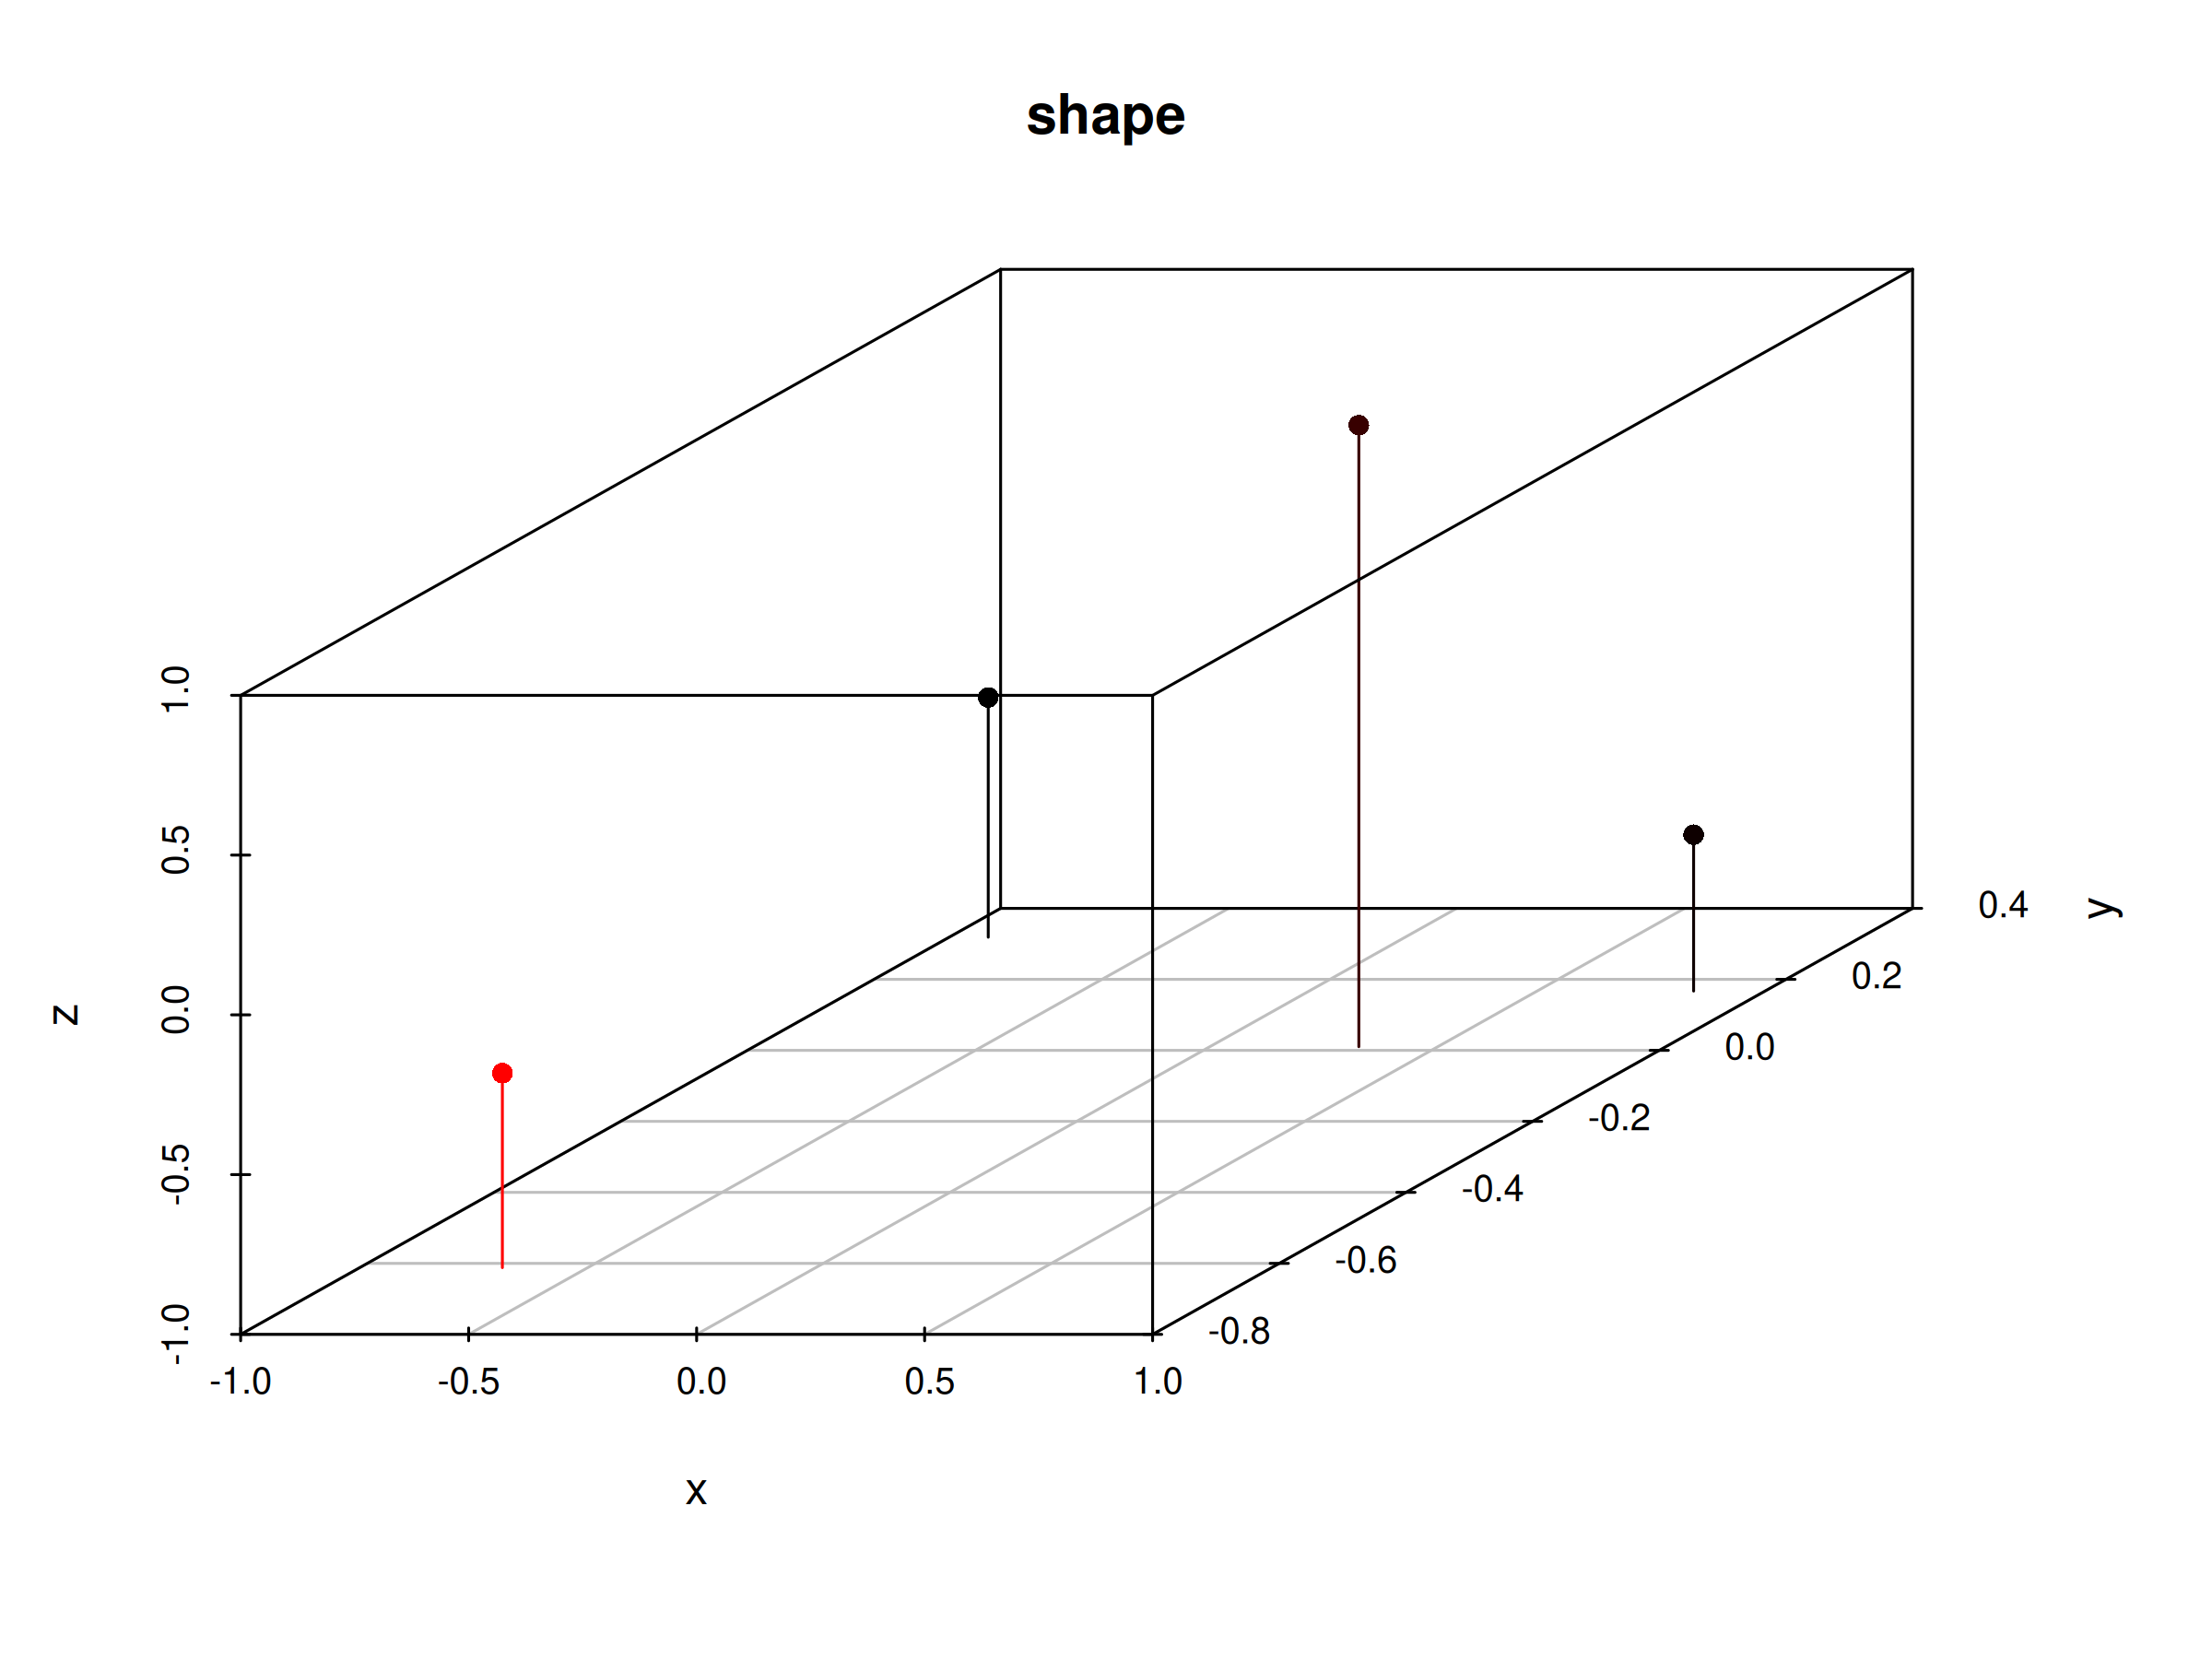
\includegraphics [width=3 in] {img/tetra.png}}
    \caption{Condition (a) Initial} \label{q1}
\end{figure}

\begin{figure}[H]
    \centerline{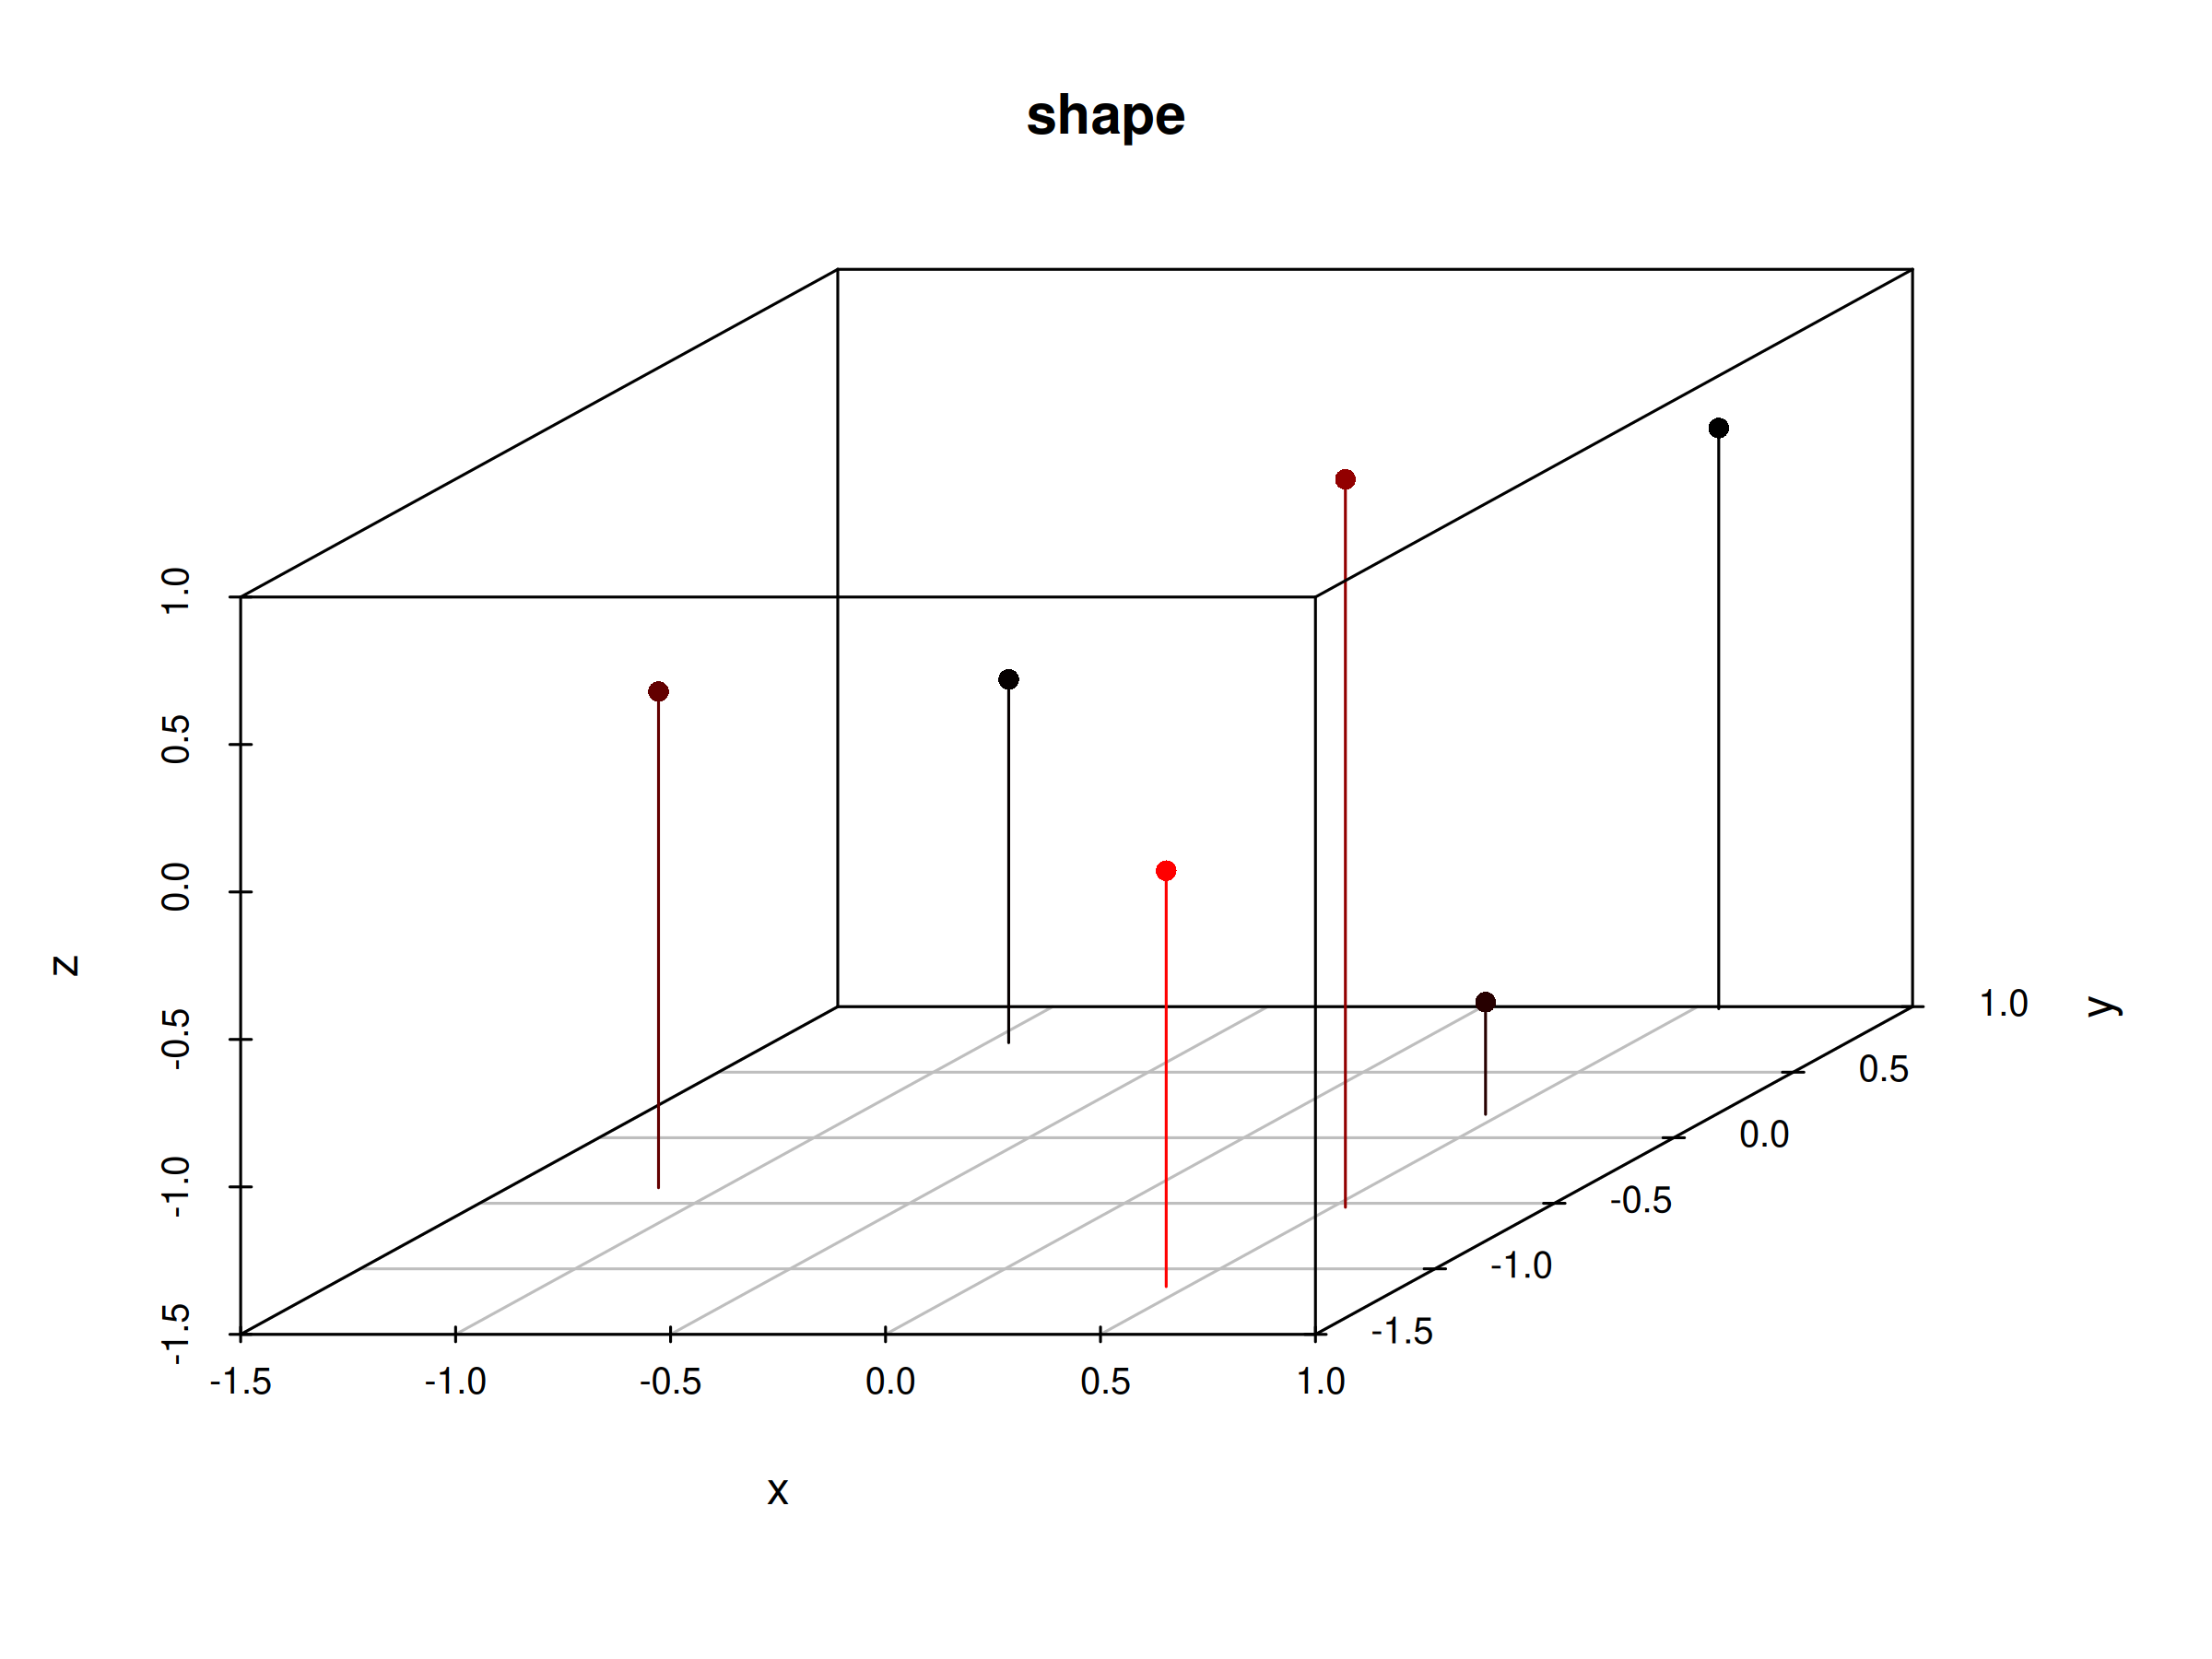
\includegraphics [width=3 in] {img/octa.png}}
    \caption{Condition (b) Initial} \label{q1}
\end{figure}

\begin{figure}[H]
    \centerline{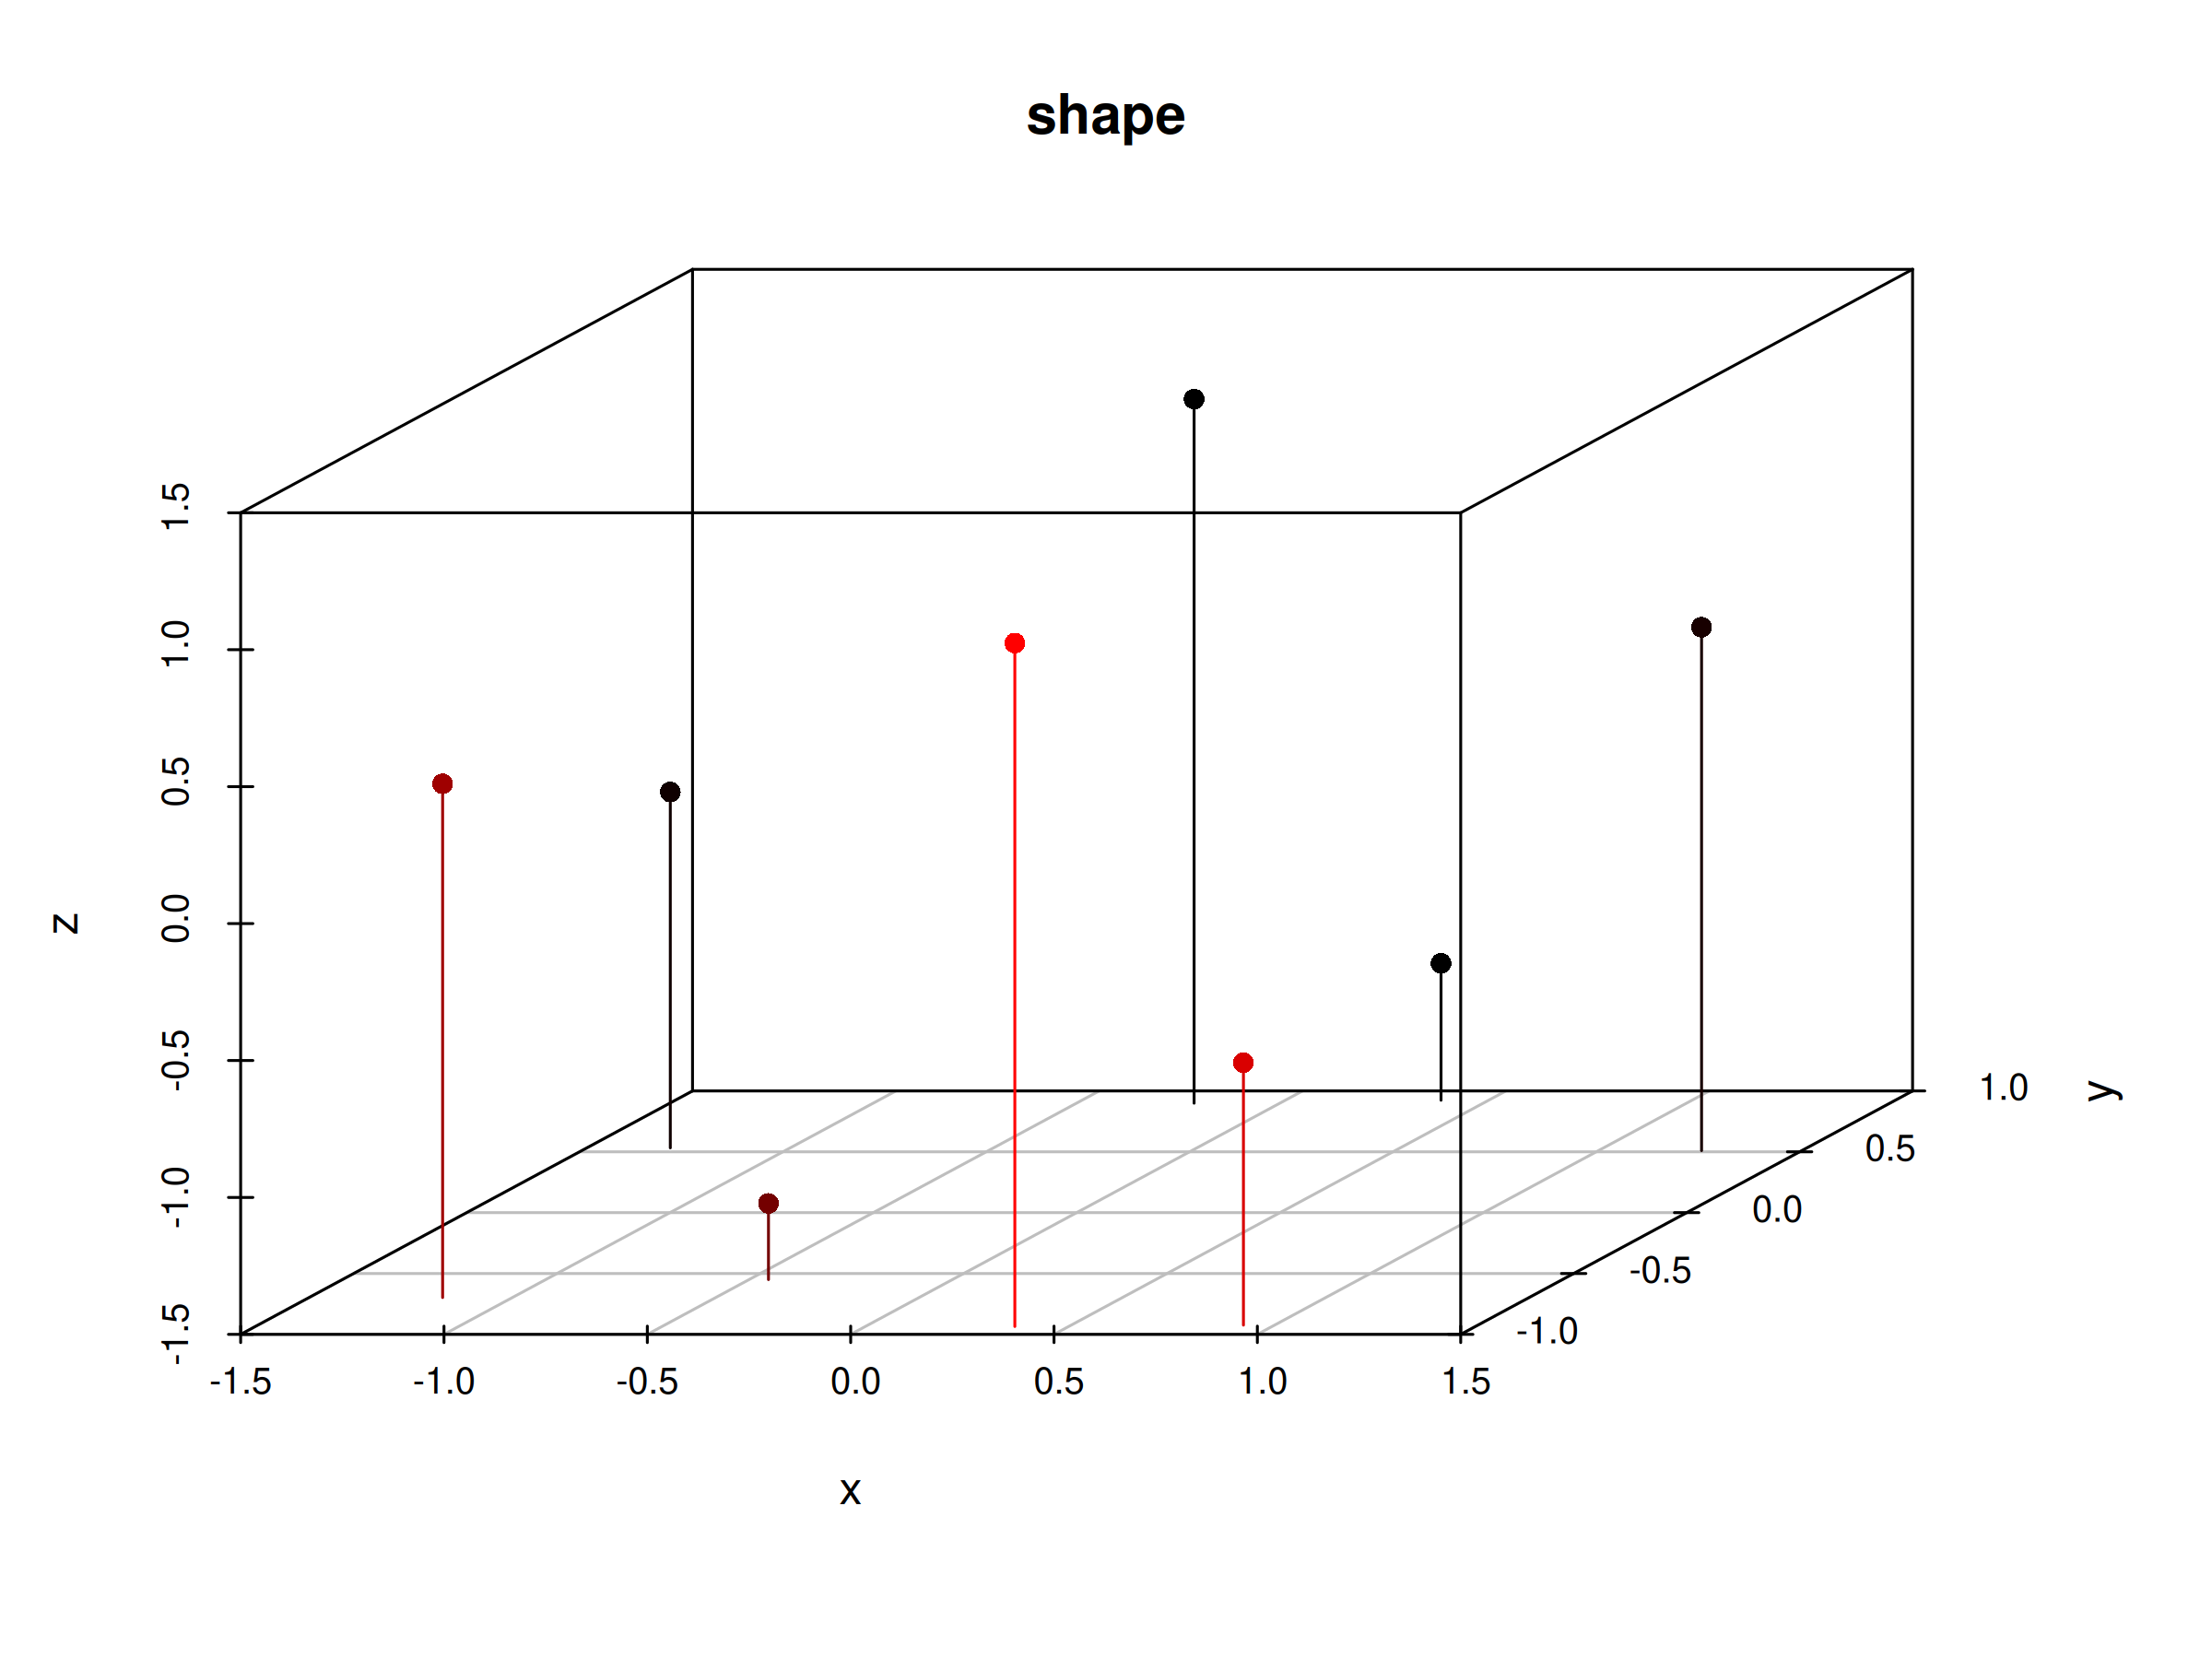
\includegraphics [width=3 in] {img/cube.png}}
    \caption{Condition (a) Results} \label{q1}
\end{figure}

\begin{figure}[H]
    \centerline{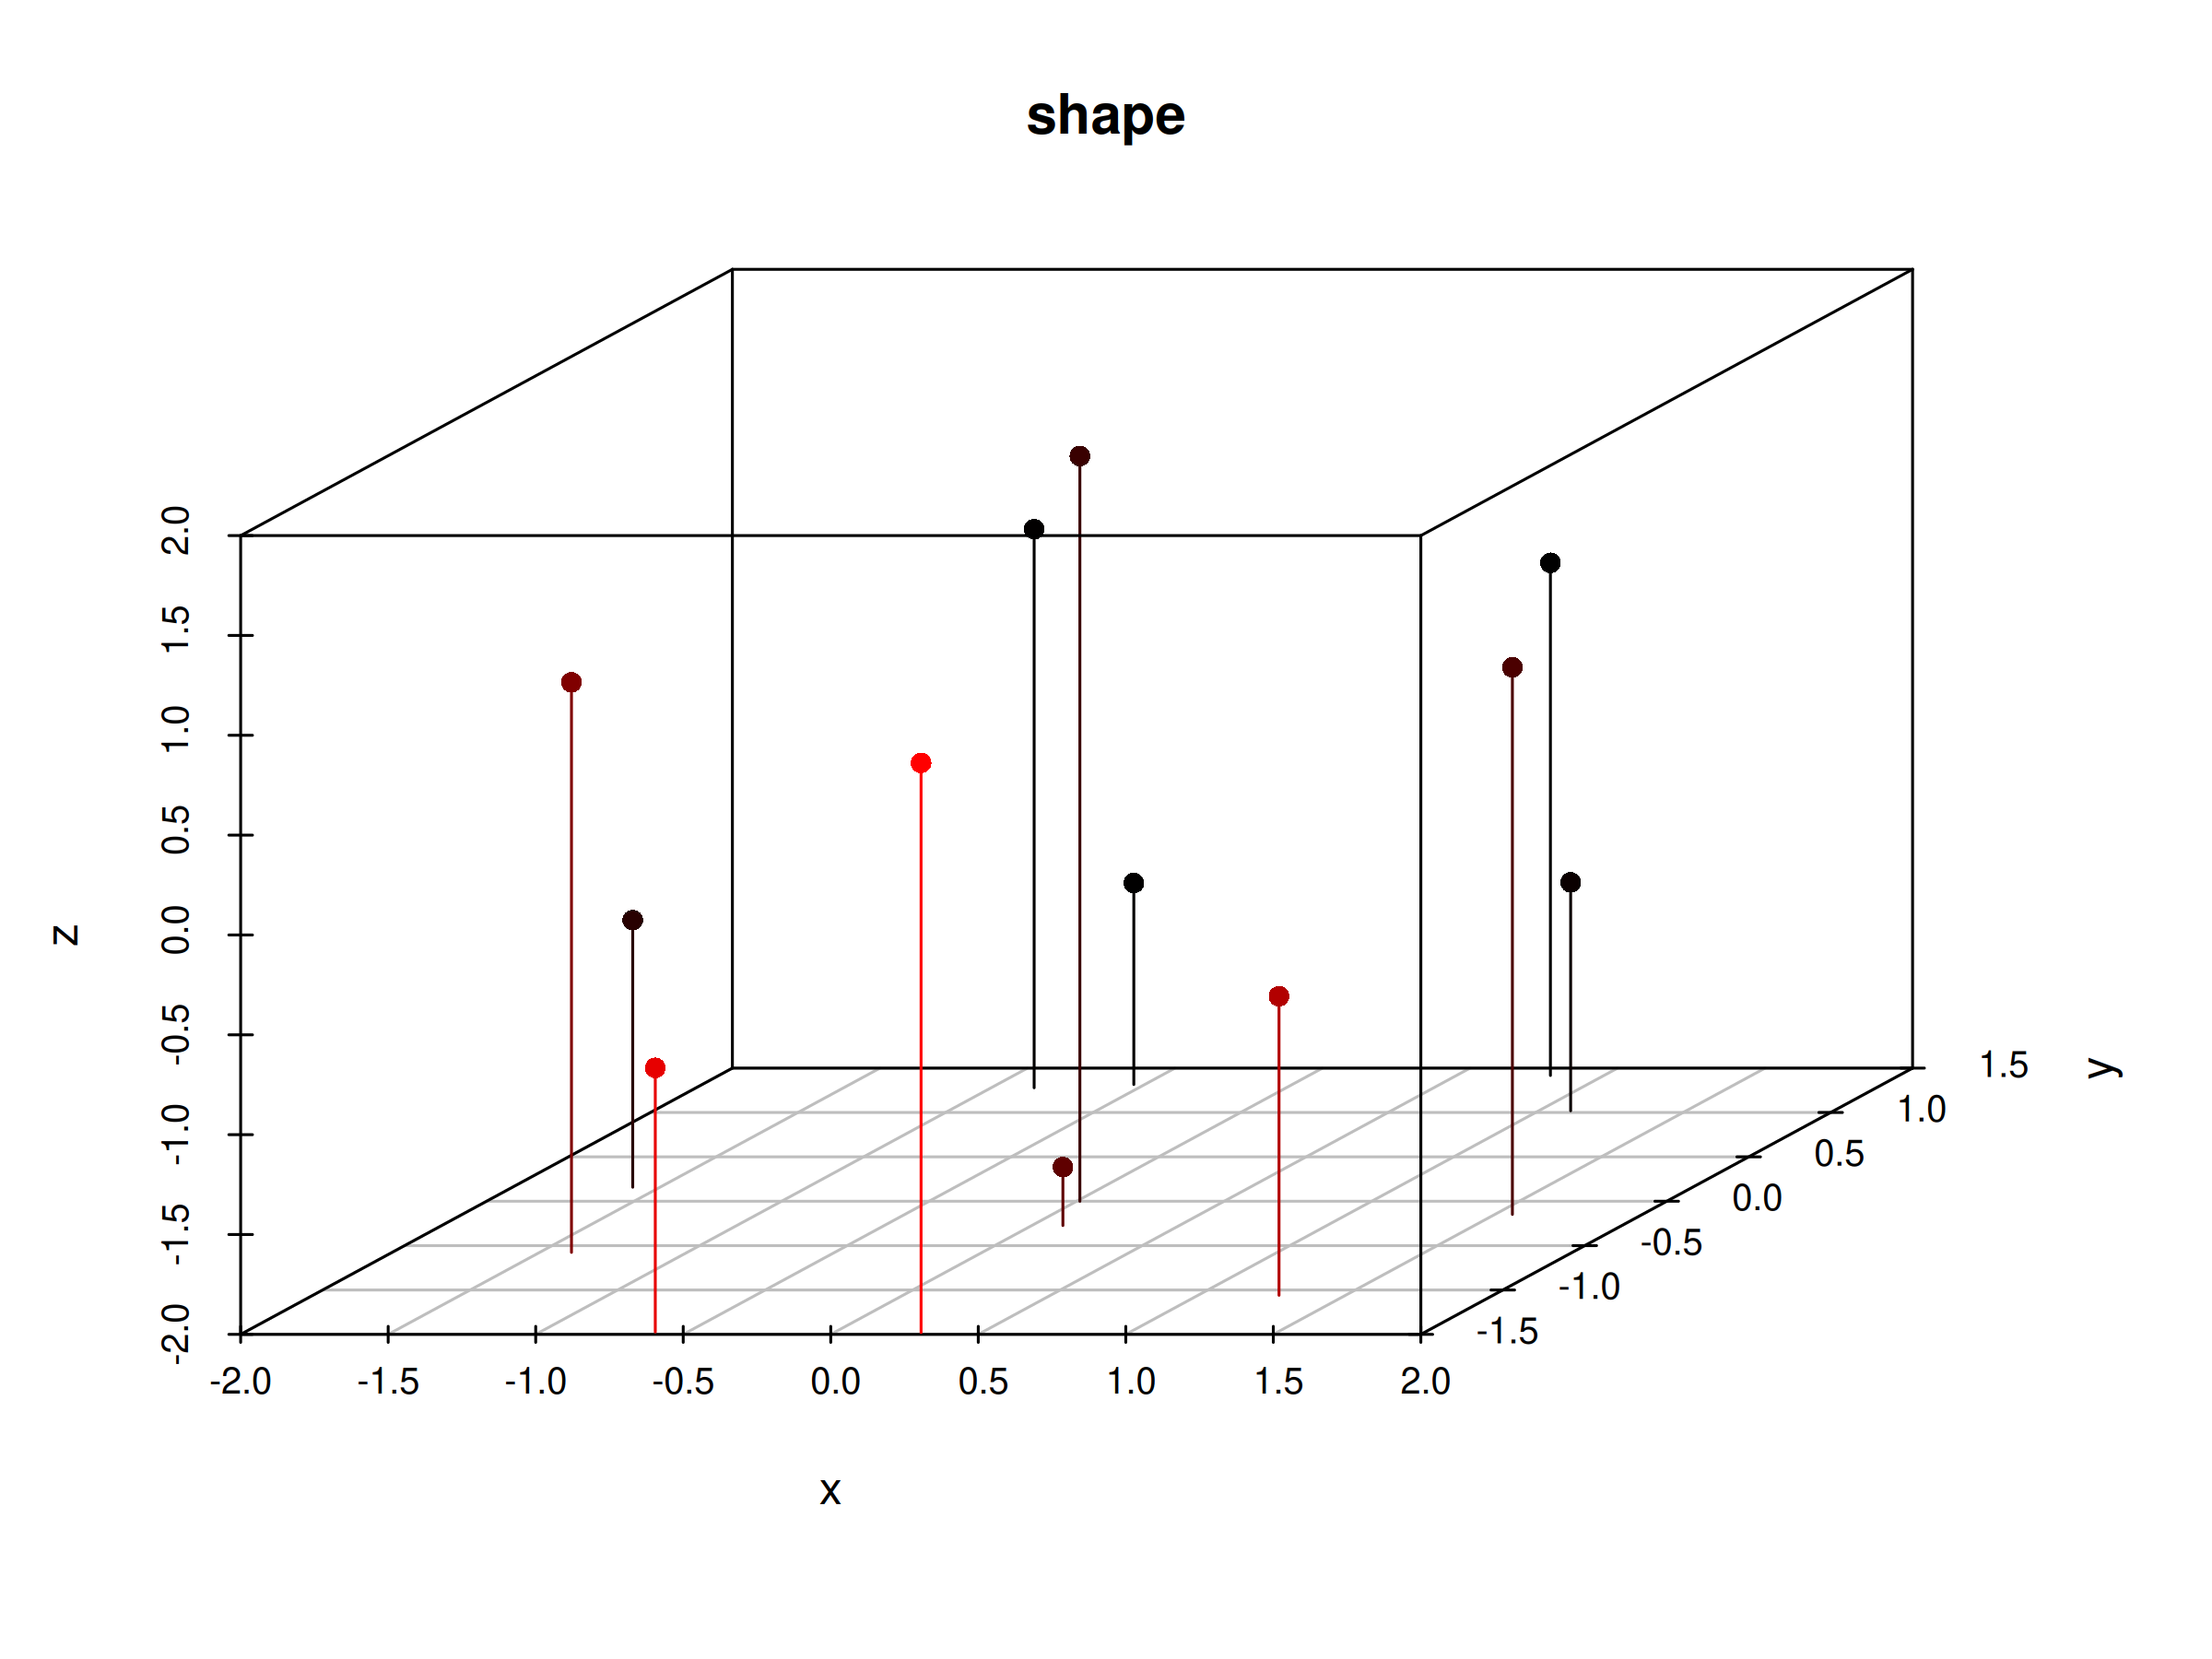
\includegraphics [width=3 in] {img/icosa.png}}
    \caption{Condition (b) Results} \label{q1}
\end{figure}

\begin{figure}[H]
    \centerline{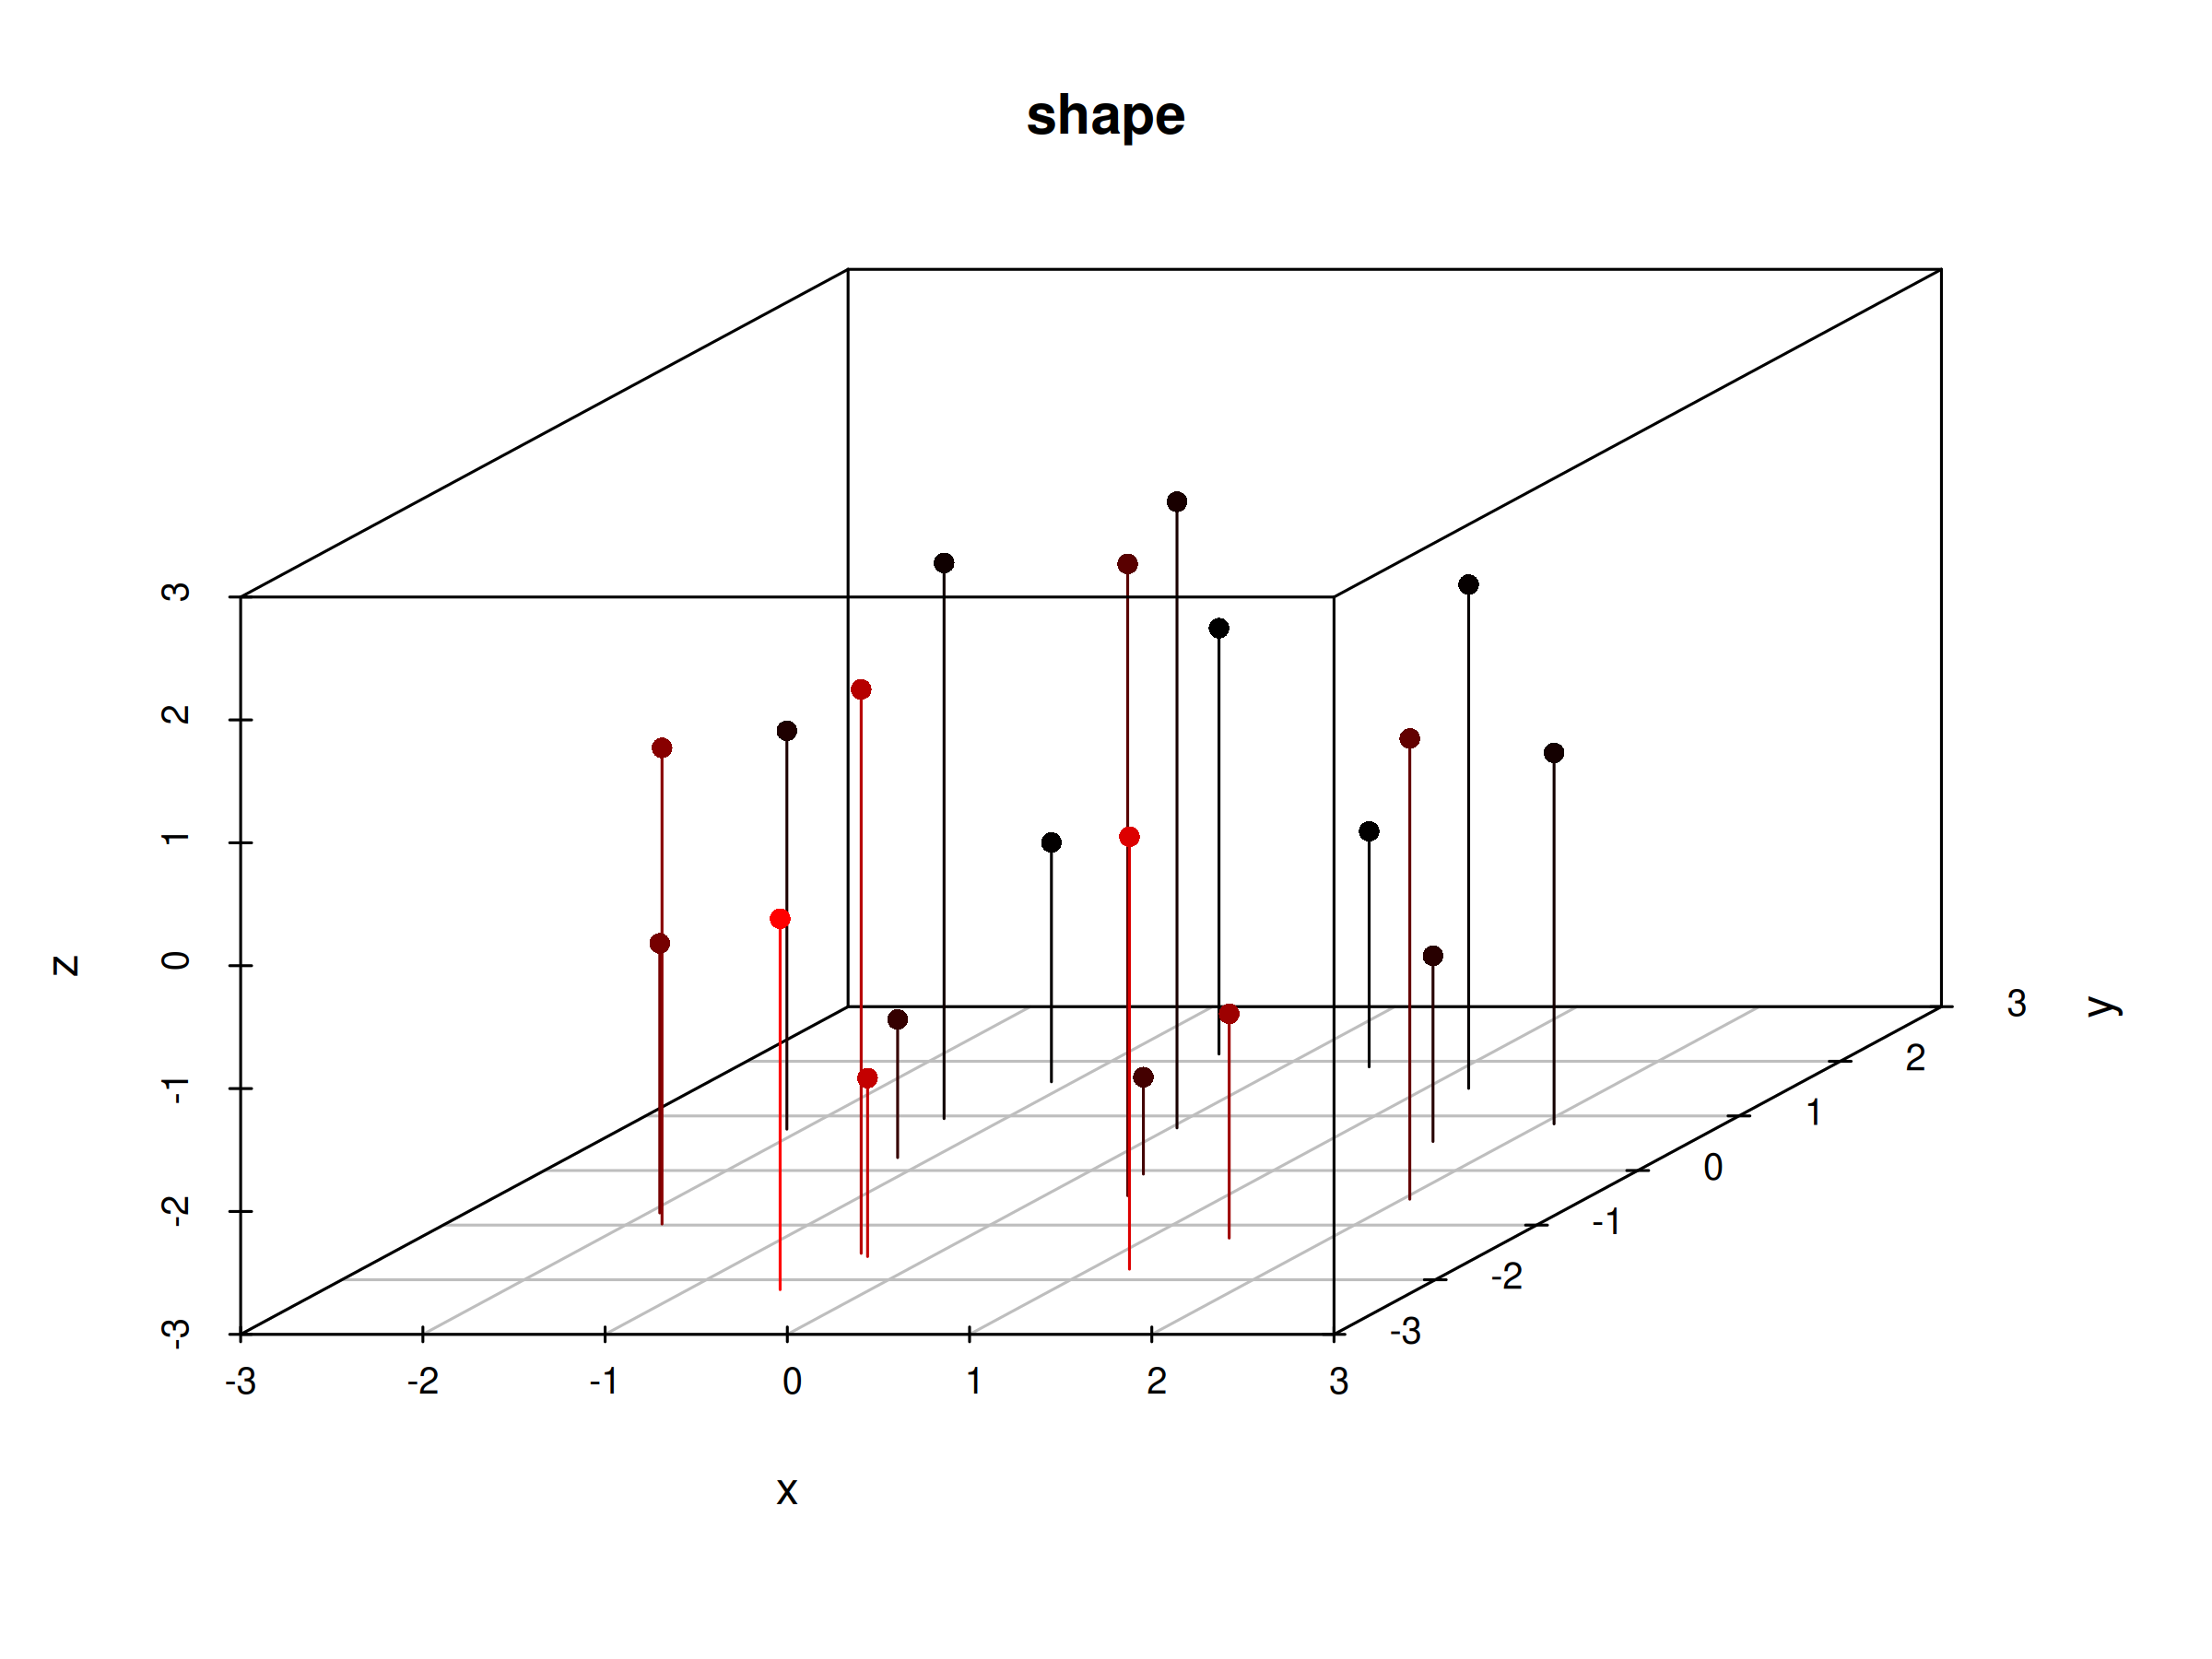
\includegraphics [width=3 in] {img/dodeca.png}}
    \caption{Condition (b) Results} \label{q1}
\end{figure}


\section{Problem 2}
\begin{thebibliography}{99}

\bibitem{thecoursetext} T. Pang, \emph{Introduction to Computational Physics},
    Cambridge University Press (2006).

\end{thebibliography}

\end{document}
